\def\tutdate{02.02.2017}
\ifdefined\compileall \else
\ifdefined\compiletype
	\documentclass[handout]{beamer}
\else
	\documentclass{beamer}
	\def\compiletype{livebeamer}
\fi

\usepackage{templates/beamerthemekitwide}

\usepackage[utf8]{inputenc}
\usepackage[T1]{fontenc}
\usepackage[ngerman]{babel}
\usepackage{listings}
\usepackage{hyperref}
\usepackage{graphicx}

\usepackage{amsmath}
\usepackage{amsthm}
\usepackage{amssymb}
\usepackage{polynom}

\usepackage{ifthen}
\usepackage{adjustbox} % for \adjincludegraphics

\newcommand{\markBlue}[1]{\textcolor{kit-blue100}{#1}}
\newcommand{\markGreen}[1]{\textcolor{kit-green100}{#1}}

\newcommand{\pitem}{\pause\item}
\newcommand{\p}{\pause}

% -- MATH MACROS
\newcommand{\thistheoremname}{}
\newcommand{\G}{\mathbb{Z}}
\newcommand{\B}{\mathbb{B}}
\newcommand{\R}{\mathbb{R}}
\newcommand{\N}{\mathbb{N}}
\newcommand{\Q}{\mathbb{Q}}
\newcommand{\C}{\mathbb{C}}
\newcommand{\Z}{\mathbb{Z}}
\newcommand{\F}{\mathbb{F}}
\newcommand{\mi}{\mathrm{i}}
\renewcommand{\epsilon}{\varepsilon}


\newenvironment<>{taskblock}[1]{%
	\setbeamercolor{block title}{fg=kit-orange15,bg=kit-orange100}
	\setbeamercolor{block body}{fg=black,bg=kit-orange30}%
	\begin{block}#2{#1}}{\end{block}}

\setbeamertemplate{enumerate items}[default]

% Aussagenlogik Symbole
\newcommand{\W}{w}
\renewcommand{\F}{f}

% Kodierung
\newcommand{\frepr}{\textbf{repr}}
\newcommand{\fRepr}{\textbf{Repr}}
\newcommand{\fZkpl}{\textbf{Zkpl}}
\newcommand{\fbin}{\textbf{bin}}
\newcommand{\fdiv}{\textbf{ div }}
\newcommand{\fmod}{\textbf{ mod }}

\title[Grundbegriffe der Informatik]{Grundbegriffe der Informatik\\Tutorium 33}
\subtitle{}
\author{Lukas Bach, lukas.bach@student.kit.edu}
\date{\tutdate}

\institute{}

\titlelogo{lukasbach}

\titleimage{bg}
%\titleimage{bg-advent}


\ifthenelse{\equal{\compiletype}{livebeamer}}
	{
		\def\livebeamermode{1}
	}{}

\ifthenelse{\equal{\compiletype}{print}}
	{
		\def\printmode{1}
	}{}

\setbeamercovered{invisible}

%\usepackage[citestyle=authoryear,bibstyle=numeric,hyperref,backend=biber]{biblatex}
%\addbibresource{templates/example.bib}
%\bibhang1em

\begin{document}
	
\selectlanguage{ngerman}


%title page
\begin{frame}
	\titlepage
\end{frame}

%table of contents
\ifdefined\printmode
	\ifdefined\compileall \else
	\begin{frame}{Gliederung}
		\tableofcontents
	\end{frame}
\fi\fi

\fi

\ifdefined\compiletype
\else
\section*{}
\begin{frame}
	\begin{itemize}
		\item Letztes Übungsblatt bis nächsten Donnerstag!
		\item Insgesamt Maximalpunktzahl aller Übungsblätter ist 206.5, also mit 103.5 hat man den Übungsschein!
	\end{itemize}
\end{frame}
\fi

\section{Automaten}
\subsection{Mealy-Automat}
\begin{frame}{Mealy-Automat}
	\begin{block}{Mealy-Automat}
		Ein Mealy-Automat ist ein Tupel $A = (Z, z_0, X, f, Y, h)$ mit...
		\begin{itemize}
			\pitem endliche Zustandsmenge $Z$
			\pitem Anfangszustand $z_0 \in Z$
			\pitem Eingabealphabet $X$
			\pitem Zustandsübergangsfunktion $f: Z \times X \rightarrow Z$
			\pitem Ausgabealphabet $Y$
			\pitem Ausgabefunktion $h: Z \times X \rightarrow Y^*$
		\end{itemize}
	\end{block}

	\pause 
	
	
	\textbf{Darstellung als Graph}\\
	\begin{itemize}
		\pitem Zustände $\rightarrow$ Knoten
		\pitem Startzustand $\rightarrow$ Pfeil an diesen Knoten (ohne Anfang)
		\pitem Zustandsüberführungsfunktion $\rightarrow$ Kanten mit Beschriftung
		\pitem Ausgabefunktion $\rightarrow$ zusätzliche Kantenbeschriftung
	\end{itemize}
\end{frame}

\begin{frame}{Beispiel Mealy-Automat}
	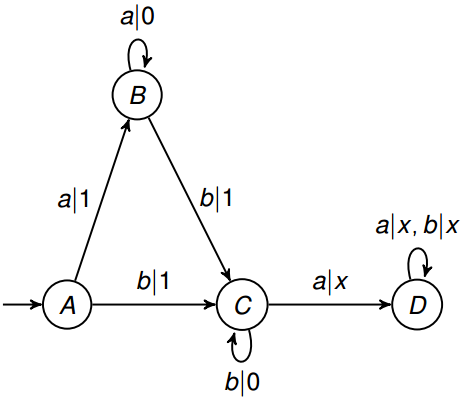
\includegraphics[scale=0.6]{images/MealyBsp.png}
\end{frame}


\subsection{Moore-Automat}

\begin{frame}{Moore-Automat}
	\pause
	\begin{block}{Moore-Automat}
		Ein Moore-Automat ist ein Tupel $A = (Z, z_0, X, f, Y, h)$ mit...
		\begin{itemize}
			\item endliche Zustandsmenge $Z$
			\item Anfangszustand $z_0 \in Z$
			\item Eingabealphabet $X$
			\item Zustandsübergangsfunktion $f: Z \times X \rightarrow Z$
			\item Ausgabealphabet $Y$
			\pitem[$\rightarrow$] \textcolor{red}{Bis hierhin alles wie bei Mealy!}
			\pitem Ausgabefunktion $h: Z \rightarrow Y^*$
		\end{itemize}
	\end{block}

	\pause
	
	\textbf{Bemerkung}\\
	Für jeden Mealy-Automaten kann man einen Moore-Automaten konstruieren, der genau die gleiche Aufgabe erfüllt, und umgekehrt.
\end{frame}

%Mal selber ausprobieren lassen
\begin{frame}{Umwandlung Mealy- in Moore-Automat}
	Links ein Mealy-, rechts ein Moore-Automat
	
	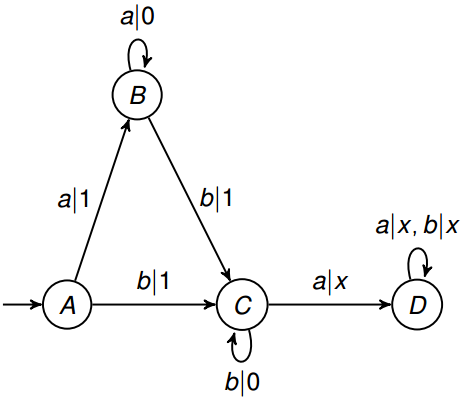
\includegraphics[scale=0.5]{images/MealyBsp.png} \pause
	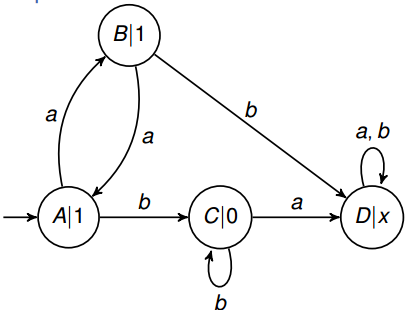
\includegraphics[scale=0.5]{images/MooreBsp.png} \pause
	
	\begin{taskblock}{Aufgabe}
		Wie sieht der Mealy-Automat als äquivalenter Moore-Automat aus, wie sieht der Moore-Automat als äquivalenter Mealy-Automat aus?
	\end{taskblock}
\end{frame}

\subsection{Endliche Akzeptoren}
\begin{frame}{Endliche Akzeptoren}
	\begin{itemize}
		\pitem Sonderfall von Moore-Automaten
		\pitem Bei einem Akzeptor will man nur wissen, ob die Eingabe akzeptiert wurde oder nicht (also reicht ein Bit als Ausgabealphabet)
		\pitem Statt der Ausgabefunktion $h$ schreibt man einfach die Menge der akzeptierenden Zustände $F \subseteq Z$ auf
		\pitem Zustände, die nicht akzeptieren, heißen ablehnend
		\pitem Im Graphen werden akzeptierende Zustände einfach mit einem doppelten Kringel gekennzeichnet 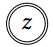
\includegraphics[scale=0.6]{images/Doppelkringel.png}
	\end{itemize}
\end{frame}

\begin{frame}{Akzeptierte Wörter und Sprachen}
	\pause
	
	\begin{block}{Akzeptierte Wörter}\p
		Ein Wort $w \in X^*$ wird vom endlichen Akzeptor akzeptiert\ip, wenn man ausgehend vom Anfangszustand bei Eingabe von w in einem akzeptierenden Zustand endet.
	\end{block}

	\pause
	
	\textbf{Bemerkung}\\
	\begin{itemize}
		\item Wird ein Wort nicht akzeptiert, dann wurde es abgelehnt
	\end{itemize}

	\pause
	
	\begin{block}{Akzeptierte formale Sprache}\p
		Die von einem Akzeptor $A$ akzeptierte formale Sprache $L(A)$ ist die Menge aller von ihm akzeptierten Wörter.
	\end{block}
\end{frame}

\begin{frame}{Endliche Akzeptoren}
	\begin{taskblock}{Aufgabe zu endlichen Akzeptoren}
		Konstruiere einen endlichen Akzeptor, der die Sprache $L_1(A) = \{w \in \{a,b\}^* : (N_a(w) \geq 3 \land N_b(w) \geq(2)\}$ erkennt.
	\end{taskblock}
	
	\pause
	\textbf{Lösung}\\
	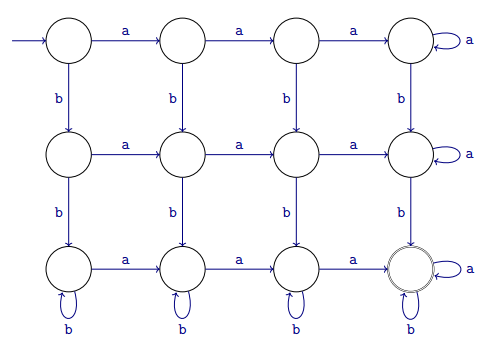
\includegraphics[scale=0.6]{images/AufgAkzeptor2.png}
\end{frame}
		
		

\begin{frame}{Endliche Akzeptoren}
	\begin{taskblock}{Aufgabe zu endlichen Akzeptoren}
		Konstruiere einen endlichen Akzeptor, der die Sprache $L_2(A) = \{w_1 ababb w_2| w_1, w_2 \in \{a,b\}^*\}$ erkennt.
	\end{taskblock}
	
	\pause
	\textbf{Lösung}\\
	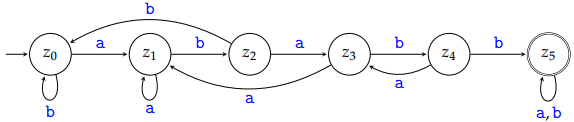
\includegraphics[scale=0.7]{images/AufgAkzeptor.png}\\
	\pause
	\begin{taskblock}{Aufgabe}
		Konstuiere einen endlichen Akzeptor der die Sprache $L_3 =\{w \in \{a,b\}^*| w \not \in L_2\}$ akzeptiert.
	\end{taskblock}
	\pause
	\textbf{Lösung} \\Ablehnende Zustände wereden zu akzeptierenden und andersrum.
\end{frame}		 

\begin{frame}{Endliche Akzeptoren}
	\begin{taskblock}{Aufgaben zu endlichen Akzeptoren}
		\begin{itemize}
			\item Gebe für den unten stehenden Automaten an, welche Sprache dieser akzeptiert.
			\item Gebe für die folgende Sprache über dem Alphabet $\{a,b\}$ einen endlichen Akzeptor an:
			$L = \{w \in \Sigma^* | N_a(w) \text{ mod } 3 > N_b(w) \text{ mod } 2\}$
		\end{itemize}
	\end{taskblock}

	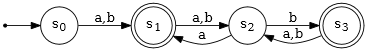
\includegraphics[scale=0.7]{images/AufgAkzeptor1.png}
\end{frame}

\begin{frame}{Lösungen}	
	\textbf{Lösung 1}\\
	$L = \{w \in \Sigma^* | |w| \text{ mod } 2 = 1\}$ (Worte ungerader Länger)\\
	\pause
	\textbf{Lösung 2}\\
	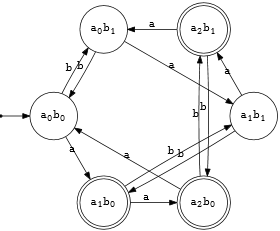
\includegraphics[scale=0.8]{images/LoesAkzeptor.png}
\end{frame}

\begin{frame}{Endliche Akzeptoren}
	Wann wird das leere Wort $\varepsilon$ von einem endlichen Akzeptor akzeptiert?\\
	\pause
	$\varepsilon \in L(A)$ gilt genau dann, wenn der Startzustand akzeptiert wird.
\end{frame}
\section{Reguläre Ausdrücke}

\begin{frame}{Regulärer Ausdruck}
	\begin{block}{Regulärer Ausdruck}
		\begin{itemize}
			\pitem Alphabet $Z = \{ |, (,), *, \emptyset\}$ von "Hilfssymbolen"
			\pitem Alphabet $A$ enthalten keine Zeichen aus $Z$
			\pitem Ein \textbf{regulärer Ausdruck} (RA) über $A$ ist eine Zeichenfolge über dem Alphabet $A \cup Z$, die gewissen Vorschriften genügt.
			\pitem Vorschriften
			\begin{itemize}
				\pitem $\emptyset$ ist ein RA
				\pitem Für jedes $x \in A$ ist x ein RA
				\pitem Wenn $R_1$ und $R_2$ RA sind, dann auch $(R_1|R_2)$ und $(R_1R_2)$
				\pitem Wenn R ein RA ist, dann auch $(R*)$
			\end{itemize}
		\end{itemize}
	\end{block}
\end{frame}

\begin{frame}{Klammerregeln}
	\begin{itemize}
		\pitem ``Stern- vor Punktrechnung''
		\pitem ``Punkt- vor Strichrechnung''
		\pitem[$\rightarrow$]$R_1|R_2R_3*$ Kurzform für $(R_1|(R_2(R_3*)))$
		\pitem Bei mehreren gleichen Operatoren ohne Klammern links geklammert
		\pitem[$\rightarrow$] $R_1|R_2|R_3$ Kurzform für $((R_1|R_2)|R_3)$
	\end{itemize}
	\pause
	\textbf{Aufgabe}\\
	Entferne so viele Klammern wie möglich, ohne die Bedeutung des RA zu verändern.\\
	\begin{itemize}
		\item $(((((ab)b)*)*)|(\emptyset*))$ \pause $\rightarrow$ $(abb)**|\emptyset*$ \pause
		\item $((a(a|b))|b)$ \pause  $\rightarrow$ $a(a|b)|b$
	\end{itemize}
\end{frame}

\begin{frame}{Alternative Definition}
	Wir können die Syntax von regulären Ausdrücken auch über eine kontextfreie Grammatik definieren. \\ \vspace{0.2cm}
	\begin{taskblock}{Aufgabe}Vervollständigt die folgende Grammatik.\end{taskblock}
	$G = (\{R\}, \{|,(,),*,\emptyset\} \cup A, R, P)$\\
	mit $P =\{R\rightarrow \emptyset, R \rightarrow \pause x \text{ }(\text{mit } x \in A),$\\$
	R \rightarrow (R|R), R \rightarrow (RR),$\\$
	R \rightarrow(R*)$\\$
	R \rightarrow \epsilon\}$
	
	\pause
	
	\vspace{.4cm} 
	Wieso brauchen wir $\epsilon$?
\end{frame}

\begin{frame}{Durch R beschriebene Sprache}
	\textbf{Notation}\\
	\begin{itemize}
		\item Spitze Klammern $\langle , \rangle$
	\end{itemize}

	\pause
	
	\textbf{Regeln}\\
	%Hier vielleicht selbst auf die Regeln kommen lassen		
	\begin{itemize}
		\item $\langle \emptyset \rangle = \pause \{\}$ \pause
		\item $\langle x \rangle = \pause \{x\}$ für jedes $x \in A$ \pause
		\item $\langle R_1| R_2\rangle = \pause \langle R_1\rangle \cup \langle R_2\rangle$ \pause
		\item $\langle R_1 R_1 \rangle = \pause \langle R_1 \rangle \cdot \langle R_2 \rangle$ \pause
		\item $\langle R* \rangle = \pause \langle R \rangle *$
	\end{itemize}
\end{frame}

\begin{frame}{Charakterisierung regulärer Sprachen}
	\begin{block}{Satz}
		Für jede formale Sprache $L$ sind äquivalent:
		\begin{enumerate}
			\item $L$ kann von einem endlichen Akzeptor erkannt werden.
			\item $L$ kann durch einen regulären Ausdruck beschrieben werden
			\item $L$ kann von einer rechtslinearen Grammatik erzeugt werden.
		\end{enumerate}
		Solche Sprachen heißten regulär.
	\end{block}
\end{frame}

\begin{frame}{Anwendung von regulären Ausdrücken}
	\vfill \centering Zum selbst probieren:\\http://regexr.com/\\\vspace{.2cm}Achtung: Reguläre Ausdrücke in praktischer Programmierung funktionieren zwar ähnlich, haben aber eine andere Syntax und können teils mehr!\vfill
\end{frame}

\section{Rechtslineare Grammatiken}
\begin{frame}{Rechtslineare Grammatiken}
	\begin{block}{Definition}
		Eine rechtslineare Grammatik ist eine reguläre Grammatik $G=(N,T,S,P)$ mit der Einschränkung, dass alle Produktionen die folgende Form haben:
		\begin{itemize}
			\item $X \rightarrow w$ mit $w \in T^*$ oder
			\item $x\rightarrow wY$ mit $w \in T^*$, $Y \in N$
		\end{itemize}
	\end{block}
\end{frame}

\begin{frame}
	\begin{taskblock}{Aufgabe zu rechtslinearen Grammatiken}
		Gebe zu $L = \{ w \in \{ 0,1 \}^* | \exists k \in \mathbb{N}_0: Num_2(w) = 2^k + 1 \}$ jeweils einen regulären Ausdruck R und eine rechtslineare Grammatik G an, sodass $L = \langle R \rangle = L(G)$ gilt.
	\end{taskblock}
	\pause
	\textbf{Lösung}\\		
	\begin{itemize}
		\item $R = (0*10)|(0*1(0)* 1) = \pause 0*10|0*10* 1 $ \pause
		\item $G = (\{S,A\}, \{0,1\}, S, \{S \rightarrow0S|10|1A, A \rightarrow 0A|1\})$
	\end{itemize}
\end{frame}

\ifdefined\compileall
\else


\ifthenelse{\equal{\compiletype}{print}}
{

\begin{frame}{Informationen}
	
	\begin{columns}
		\begin{column}{0.5\textwidth}
			
			\begin{block}{Zum Tutorium}
				\begin{itemize}
					\item Lukas Bach
					\item Tutorienfolien auf: 
					\begin{itemize}
						\item \url{http://gbi.lukasbach.com}
					\end{itemize}
					\item Tutorium findet statt:
					\begin{itemize}
						\item Donnerstags, 14:00 - 15:30
						\item 50.34 Informatikbau, -107
					\end{itemize}
				\end{itemize}
			\end{block}
			
			\begin{block}{Mehr Material}
				\begin{itemize}
					\item Ehemalige GBI Webseite:
					\begin{itemize}
						\item \url{http://gbi.ira.uka.de}
						\item Altklausuren!
					\end{itemize}
				\end{itemize}
			\end{block}
			
		\end{column}
		\begin{column}{0.5\textwidth}
			
			\begin{block}{Zur Veranstaltung}
				\begin{itemize}
					\item Grundbegriffe der Informatik
					\item Klausurtermin:
					\begin{itemize}
						\item 06.03.2017, 11:00
						\item Zwei Stunden Bearbeitungszeit
						\item 6 ECTS für Informatiker und Informationswirte, 4 ECTS für Mathematiker und Physiker
					\end{itemize}
				\end{itemize}
			\end{block}
			
			\begin{block}{Zum Übungsschein}
				\begin{itemize}
					\item Übungsblatt jede Woche
					\item Ab 50\% insgesamt hat man den Übungsschein
					\item Keine Voraussetzung für die Klausur, aber für das Modul
				\end{itemize}
			\end{block}
			
		\end{column}
	\end{columns}
	
\end{frame}

}{}

\ifdefined\livebeamermode
	\begin{frame}
		
\includegraphics[width=\linewidth]{images/thatsall.png}
	\end{frame}
\fi

\end{document}

\fi